\section{Open and reproducible science}

Scientific data is hard to get by request, even for editors. In an editorial for the neuroscience journal Molecular Brain, \textcite{Miyakawa2020-ze} described his experience with asking authors for raw data. Out of the $180$ submissions he handled, he made $41$ requests for raw data as part of a ``Revise before review'' decision. Among these $41$ manuscripts, $21$ withdrew their submission. Out of the $20$ manuscripts left, Miyakawa rejected $19$ due to insufficient raw data. Thus $97\%$ of the submissions failed to provide raw data of good quality even after a request. Miyakawa suggests the possibility ``that the raw data did not exist from the beginning, at least in some portions of these cases.''

Data is even harder to get for non-editors. As part of a study of psychological research's robustness to outliers, \textcite{Wicherts2006-yy} requested data from $141$ research psychologists, but received some data from only $27\%$ percent of them. This was not plausibly because the data was lost: All of the papers they requested data from were published during the last $12$ months. Moreover, the contacted psychologists reneged on their duty. All of them had signed the American Psychological Association's $2001$ ethics code, which contains the sentence ``psychologists do not withhold the data on which their conclusions are based from other competent professionals'' \parencite[p. 396; as cited in Wicherts et al. 2006][]{American_Psychological_Association2001-rs}. 
\textcite{Wicherts2006-yy} are not the only researchers who have had trouble getting data. \cite[p. 526]{Nelson2018-ov} wrote: 
\begin{quote} Requesting data from another researcher---particularly for the stated justification of suspecting fraud---is socially taxing. Furthermore, although the APA prescribes the sharing of data, there is no enforcement mechanism. We have heard many stories from other researchers who were told that the requested data were coming soon (but then never arrive), were impossible to share, had been lost, or were legally impounded. We have personally been denied data explicitly because the authors wished to avoid criticism; the authors wrote bluntly, \textquotedblleft no data for you.''
\end{quote}
There are some valid reasons not to share data. Most important is the issue of privacy, where there are both ethical and legal issues. But for the majority of psychology papers, the reasons not for sharing data are bad. It is natural to suspect that data is withheld since the authors want to avoid criticism or scrutiny, and there is some evidence for this suspicion. Using the data from the aforementioned study of \textcite{Wicherts2006-yy}, \textcite{Wicherts2011-eb} argue that the reluctance to share data is associated with the study's quality. For instance, $25\%$ of the studies that did not share data reported \textit{p}-values below $0.05$ when they were not, in fact, below $0.05$; this error was not committed by any of the studies that shared data.

The benefits of sharing data are numerous, and not always obvious. \textcite{Wicherts2012-cp} lists six points. First, sharing data preserves it. If you keep your data only on your own computer, it will eventually be lost. Second, openness allows other researchers to independently reproduce your results. They can uncover errors in the analysis, \emph{p-}hacking, or scientific misconduct. Third, publishing data can make the paper more citeable. This is especially relatable for methodologists, who frequently cite papers only since they are associated with data sets. Fourth and fifth, other researchers can run different analysis on your data. For statisticians this one is an obvious one, and is especially important for meta-analysists \nptextcite{Cooper2009-ge}. Finally, founding agencies routinely stipulate that data must kept in an accessible form for some minimum amount of years. If the data are made open, you do not have to worry at all about this.  

A major reason to demand open data is to prevent scientific fraud. While most researchers believe that fraud is uncommon, it is extremely difficult to measure. Since there are strong incentives to falsify data and incorrectly report summary statistics, it is imprudent to assume no one does it. Demanding open data reduces the number of fraudulent papers by two mechanism. First, you are strongly disincentivized to falsify data and summary statistics when the data are publicly available. For other researchers can, in principle, uncover your fraud at any moment. Second, fraudulent papers will be uncovered at a greater rate when the evidence is available for scrutiny. By merely looking at reported standard deviations and means, \textcite{Simonsohn2013-ul} started to suspect two authors of systematic data manipulation. Luckily, the authors supplied him with the raw data, which only strengthened the suspicion of fraud. One of the authors, Dirk Smeesters, has now been convicted of scientific misconduct. The other, Lawrence Sanna, suddenly resigned from his professorship. However, \textcite{Simonsohn2013-ul}
also observed a ``third case of exceedingly similar summary statistics''. Sadly, he did not get hold of the data, as the ``main author reported losing them, and the coauthors of the article did not wish to get involved''.

Sharing data is just one part of open and reproducible science. It is equally important to share the code employed in the preparation of the manuscripts. The code should be readable, that is, no spaghetti code, documented, and preferably tested. Even better, the code should be integrated with the manuscript itself, allowing a compilation of a single file to reproduce the entire manuscript. The $\mathtt{R}$ environment provides tools to do such reproducible science, most importantly \texttt{rmarkdown} \nptextcite{Xie2018}.

The reasons to share code are pretty much the same as the reasons to share data. Openness fosters better research and invites scrutiny for other researchers. It increases the trust in your research. It probably fosters collaboration too; it is much easier to approach someone about what they do when you know what they are doing.

Papers report inconsistent statistics. \textcite{Nuijten2016-eu} reports that one of two psychology papers contains \emph{p}-values that are inconsistent with its reported test statistics. Moreover, one of eight papers have gross inconsistencies, where a reported \emph{p}-value is significant but its computed \emph{p}-value is not. As a reader without access to either the data or the code used to calculate the statistics, you are left in the dark about what the data actually says.

\textcite{John2012-xp} measured the frequency of \emph{p}-hacking and other questionable research practices, in psychology using an electronic survey. Figure \ref{fig:john2012} shows their results. Most of these questions are about \emph{p}-hacking, but question eight is about \emph{hypothesising after results are known} (denoted \emph{HARKing} by \textcite{Kerr1998-by}), and question ten about scientific fraud. Approximately one third of the respondents admitted to hypothesising after results are known. Doing this certainly makes \emph{p}-values invalid, as choosing a null hypothesis conditioned its \emph{p}-value being less than $0.05$ definitely makes you reject the null hypothesis. But hypothesising after results are known is detrimental for other reasons too, and \cite[p. 205]{Kerr1998-by} lists nine additional reasons why.

\begin{figure}
\noindent \begin{centering}
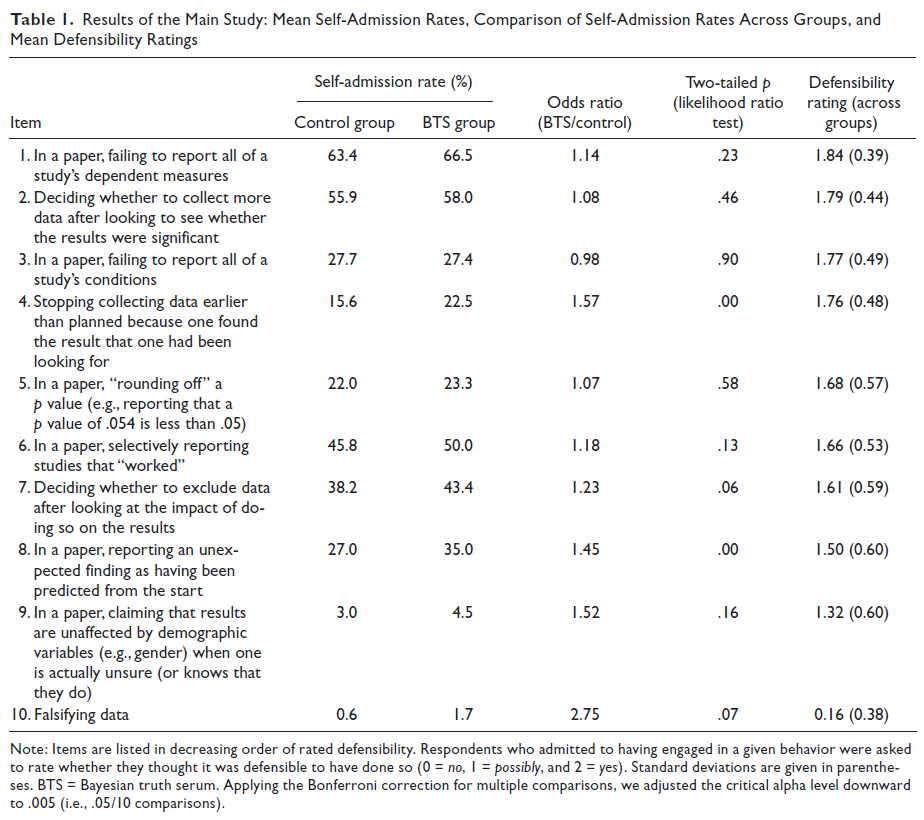
\includegraphics[scale=0.4]{chunks/john2012}
\par\end{centering}
\caption{\label{fig:john2012}Self-admission rates to questionable research practices from \textcite{John2012-xp}. The participants in BTS group were given incentives for honest reporting, and the defensibility rating indicates how defensible the respondents consider each practice to be.}
\end{figure}

A study is preregistered if it is planned in detail in advance and the this plan is publicly known \nptextcite{Van_t_Veer2016-fo}. The plan should include the what hypotheses are tested, the experimental methods used, and an exact specification on the statistical analysis. A benefit of proper preregistration is that it makes hypothesising after results are known impossible, which on its own should reduce the rate of false positives in the literature quite a bit. But preregistration is also a remedy for \emph{p}-hacking, and can even help with publication bias.

\textcite{Scheel2020-sq} studied rate of positive results in standard research versus preregistered research. Among $148$ standard, non-preregistered studies sampled, $142$ were positive. That is, $95\%$ were positive. On the other hand only $15/30=50\%$ of the preregistered reports were positive. Such a rate of positive results is far more plausible than $95\%$, especially when seen in light of the fact that most psychological research is severely underpowered \nptextcite{Sedlmeier1989-zz}.

\subsection{Open science, $\mathtt{R}$, and statistics}

\texttt{R} is not only a popular language among statisticians, but among other scientists as well, in particular social scientists and biologists. The \texttt{R} community is full of dedicated user, with roughly $16,000$ \texttt{CRAN} packages as of writing. Most \texttt{R} package development takes place on Github or other git-based platforms such as Gitlab. These platforms allow for version control, code sharing, collaboration, and issue tracking. Lately, it has become more popular to collaborate on papers on this papers as well, often with \texttt{R} taking the center spot.

There are high-quality tools that greatly simplify the production of high-quality $\mathtt{R}$ code. Some of the most important are $\texttt{devtools}$ \nptextcite{devtools}, for creating and disseminating $\mathtt{R}$ packages, $\mathtt{Roxygen}$ \nptextcite{roxygen2} for automatized creation of documentation. The packages \texttt{knitr} \nptextcite{Xie2014} and R markdown allows you to create manuscripts, blog posts, $\mathtt{R}$ package vignettes, reports, and even Beamer presentations without leaving $\mathtt{R}$.

Several $\mathtt{R}$ packages aid researchers in doing open and reproducible science in $\mathtt{R}$. The \texttt{codebook} package by \textcite{Arslan2019-tg} assists in creating documentation for data sets. The packages \texttt{xtable} \nptextcite{xtable} and \texttt{huxtable} \nptextcite{huxtable} creates Latex tables from $\mathtt{R}$ code. \texttt{renv} \nptextcite{renv} and \texttt{packrat} \nptextcite{packrat} manages package version so that the code used to run the analysis does not break do to changes in external packages. The package \texttt{papaja} \nptextcite{papaja} makes knitr documents adhere to popular the American Psychological Association (APA) style. $\mathtt{worcs}$ \nptextcite{Van_Lissa2020-sb} is a template for open science in $\mathtt{R}$ developed by psychologists. This is just a small selection of packages for open and reproducible research.

Documentation allows the user to use the software without guessing what it does. Ideally, the user will understand what your code does without having to read your code at all. And in this sense, high-quality documentation lowers the bar for both users and contributors to engage with your code and understand your research. Documentation forces you think about how general your function is, what its input should be, and as a consequence, what it can be used for. As a consequence, documentation leads to better code. When you revisit your code $4$ years from now, you can actually read it and understand what it does. 

An essential part of a high-quality coding project are \emph{formal tests}, or tests that are purposefully designed to make sure your code does what it should. Formal testing of code has plenty of benefits. First and foremost, testing increases the quality of your code. According to \cite[Chapter 7]{Wickham2015-ik}, testing causes bugs to disappear, better code structure, and more robust code. An R package with plenty of formal tests can be trusted more than one without tests. That tests have been written and passed demonstrates the program does at least something correctly, provided the tests are well-written. Second, tests inspire confidence in the authors. An author who carefully writes tests is less sloppy that one who cannot find the time to or does not bother. Third, since tests make code better, the code can be trusted to work well too. An especially good practice for $\mathtt{R}$ packages is to cross-check the output of functions. For instance, the $\mathtt{R}$ time series package \texttt{memochange} \nptextcite{memochange} checks the output of every function against outputs in the literature.

R packages are accessible and often easy to use, which makes it possible for other people to find errors and correct your mistakes. If you multiply by $2$ instead of $\sqrt{2}$ and don't make the code public, you will never know. Most methods development is exploratory, and works by carefully experimenting with different setups, starting with the well-known then slowly proceeding to the more difficult. High-quality R packages helps your colleagues do their research, since they can build, incrementally, on your trusted work.  

You can trust mathematical results to the extent you and your colleagues can verify the proofs. Importantly, a good proof should be relatively cheap to verify in terms of time and effort. This is a strong incentive for writing correct proofs. Simulations, however, are usually a chore to write and to verify. We only do them because we have to. Probably no one will try to replicate them. To make simulations, custom Markov chain Monte Carlo samplers, and similar difficult programs worth considering seriously, the code should be both documented, tested, and open. For why should be expect statisticians to behave better than psychologists? 

Sharing code can make a difference even when using the best-known methods. \textcite{McCullough2003-zd} discusses how the coefficients of a Probit regression couldn't be reproduced. In their, case the irreproducibility occurred since the likelihood didn't have a maximum, but the numerical algorithm failed to inform the user that a maximum wasn't found. The authors go on to describe how one can, through force of labour, verify or disconfirm that a proposed maximum is in fact a maximum. Considering that many, if not the majority, of research statisticians are not specialists in numerical analysis, it is irrational to expect every statistician to write perfect numerical solvers for every maximization problem he studies. Since sharing well-documented code makes it much easier for researchers to scrutinize your work, problems such as non-sensical estimates are far more likely to be uncovered.

In the Transparency and Openness Promotion guidelines \nptextcite{Nosek2015-hh}, the highest level of analytical openness states that ``Code must be posted to a trusted repository, and reported analyses will be reproduced independently before publication.''. At the time of writing, 26 journals adhered to this code according to https://topfactor.org/. Such strong codes were even enforced by some journals years ago according to \textcite{Nosek2015-hh}, who states that ``the journals Political Analysis and Quarterly Journal of Political Science require authors to provide their code for review, and editors reproduce the reported analyses publication. ``

How does statistical journals compare? I checked the instructions to authors pages of seven top journals to find out. \emph{Biometrika} encourages authors to provide code and data, but does not require it, as ``Biometrika strongly encourages authors to make all data and software code on which the conclusions of the paper rely available to readers.'' The Journal of the American Statistical Society, similarly,``[...] strongly encourages all authors to submit datasets, code, other programs, and/or extended appendices that are directly relevant to their submitted articles, [...].'' \emph{Journal of the Royal Statistical Society, Series B}, has a slightly less ambiguous statement, namely that ``it is the policy of the Journal of the Royal Statistical Society that published papers should, where possible, be accompanied by the data and computer code used in the analysis. Both data and code must be clearly and precisely documented, in enough detail that it is possible to replicate all results in the final version of the paper.'' The Journal of Graphical and Computational Statistics has the strongest demand, stating that ``Authors are expected to submit code and datasets as online supplements to the manuscript. Exceptions for reasons of security or confidentiality may be granted by the Editor. `` The journals \emph{Annals of Statistics}, \emph{Electronic Journal of Statistics}, and \emph{Bayesian Analaysis} say nothing about code and data in their instructions to authors pages.
